\documentclass[preprint]{revtex4-1}
\usepackage{graphicx}
\usepackage{epstopdf}
\usepackage{amsmath}
\usepackage{hyperref}
\usepackage{booktabs}
\usepackage{color}

\usepackage{SIunits}
\newcommand{\wstar}{-0.023}
\newcommand{\Qstar}{0.25}

\setlength{\tabcolsep}{10pt}

\newenvironment{sistema}%
  {\left\lbrace\begin{array}{@{}l@{}}}%
  {\end{array}\right.}


\usepackage{pgfplots}
\usepgfplotslibrary{external}
\usepgfplotslibrary{groupplots}
\usetikzlibrary{positioning}
\usetikzlibrary{plotmarks}
\tikzexternalize
\tikzset{external/force remake}
\tikzset{every mark/.append style={scale=0.8}}
\pgfplotsset{every axis/.append style={small}}

\begin{document}
\tikzset{external/force remake=false}
\begin{figure}
	\centering
	\begin{tikzpicture}[
		pic3d/.style={inner sep=0}, %
		lab/.style={above right, text height=0.8em, text depth=0.2em, font=\Large\bfseries}%
		]%
		\node[pic3d] (m3d) {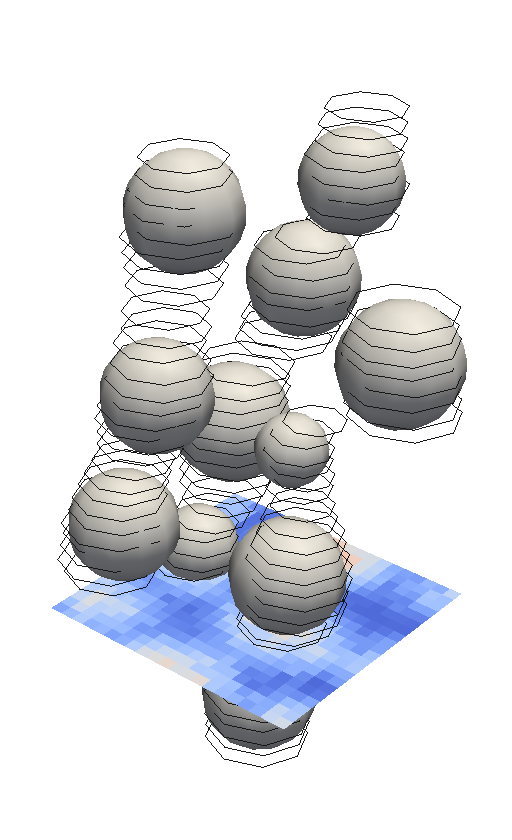
\includegraphics[width=0.28\textwidth]{comp2D3D_crop}};
		\node[lab] at (m3d.south west) {a};
		\node [pic3d, right] at (m3d.east) (m2d) {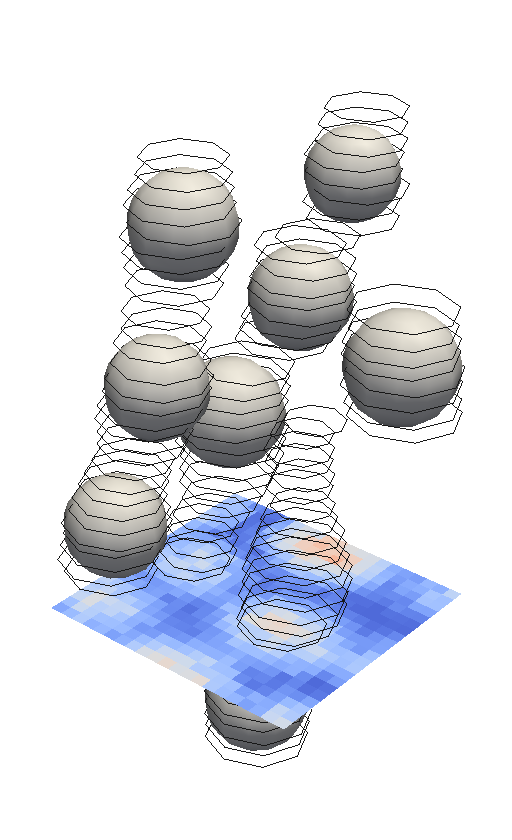
\includegraphics[width=0.28\textwidth]{comp2D_reconstructed_crop}};
		\node[lab] at (m2d.south west) {b};
		\node [pic3d, below right] at (m2d.north east) (cg20) {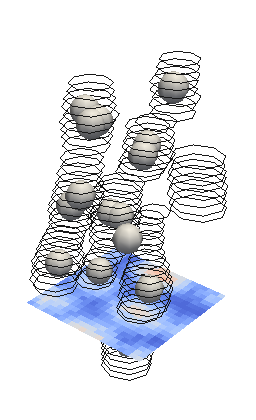
\includegraphics[width=0.14\textwidth]{comp3D_monoscale_r20_crop}};
		\node[lab] at (cg20.south west) {c};
		\node [pic3d, right] at (cg20.east) (cg25) {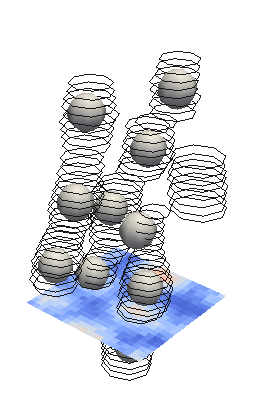
\includegraphics[width=0.14\textwidth]{comp3D_monoscale_r25_crop}};
		\node[lab] at (cg25.south west) {d};
		\node [pic3d, right] at (cg25.east) (cg30) {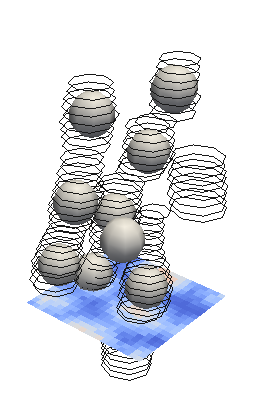
\includegraphics[width=0.14\textwidth]{comp3D_monoscale_r30_crop}};
		\node[lab] at (cg30.south west) {e};
		\node [pic3d, above right] at (m2d.south east) (cg35) {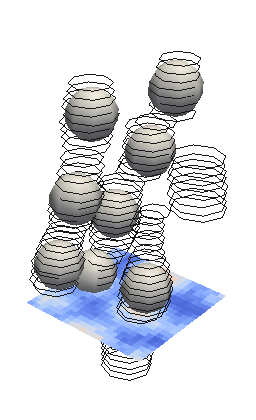
\includegraphics[width=0.14\textwidth]{comp3D_monoscale_r35_crop}};
		\node[lab] at (cg35.south west) {f};
		\node [pic3d, right] at (cg35.east) (cg40) {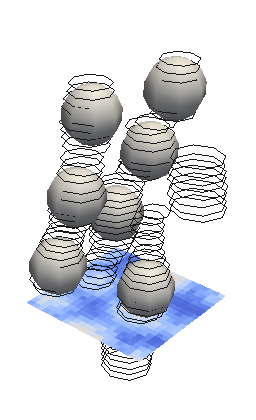
\includegraphics[width=0.14\textwidth]{comp3D_monoscale_r40_crop}};
		\node[lab] at (cg40.south west) {g};
		\node [pic3d, right] at (cg40.east) (cg45) {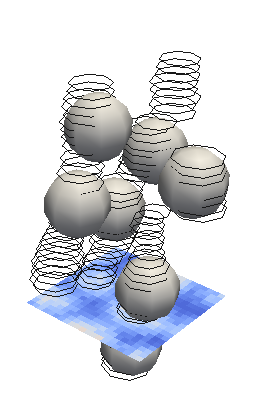
\includegraphics[width=0.14\textwidth]{comp3D_monoscale_r45_crop}};
		\node[lab] at (cg45.south west) {h};
	\end{tikzpicture}
	\caption{\textbf{Visualisation of the results of various tracking methods for the same portion of image.} \textbf{a} Multiscale 3D tracking. \textbf{b} Reconstruction from 2D tracking. \textbf{c-h} Crocker and Grier in 3D with blurring radius increasing from \unit{2}{px} to \unit{4.5}{px} by steps of \unit{0.5}{px}. The circles on each picture are the result of 2D multiscale tracking of each XY slice of the 3D pictures. Sphere are displayed with radii determined by the tracking methods in \textbf{a-b}, and equal to the blurring radius for \textbf{c-h}.}
	\label{fig:result3d}
\end{figure}
\tikzset{external/force remake=false}
\begin{figure}
	\centering
	\begin{tikzpicture}[lab/.style={below left, text height=0.8em, text depth=0.2em, font=\Large\bfseries}]
	\begin{axis}[%
		name=hist,
		width=0.45\textwidth,%
		%scale only axis,
		xmin=1, xmax=5,
		axis y line*=left,
		ymin=0, ytick=\empty,%
		ylabel={Size distribution (a.u.)},%
		ylabel near ticks,
		]
		\addplot[ybar, ybar interval] file {SEM_size_distrib.txt};
	\end{axis}
	\begin{axis}[%
		%scale only axis,
		width=0.45\textwidth,%
		xmin=1, xmax=5,
		axis y line*=right,
		xlabel={Diameters [$\micro\metre$]},%
		ymin=0, ytick=\empty,%
		no marks,%
		]
		\addplot+[dashed] file {go1_intensity.sizes};
		\addplot table [x expr ={\thisrowno{0}/1.23}, y index=1] {go1_intensity.sizes};
		\draw[->, ultra thick] (axis cs:3.15,0.05) -- (axis cs: 3.9, 0.05) node[right] {swelling};
		\node[lab] at (rel axis cs:0.95,0.95) {a};
	\end{axis}
	\node[right=3em of hist.right of south east] (a){};
	\begin{axis}[%
		at=(a),
		anchor=south west,%
		width=0.45\textwidth,%
		xmin=0, xmax=1.5,%
		xlabel ={$r/\left\langle \sigma\right\rangle$, $\hat{r}$},%
		ymin=0,%
		ylabel=$g(r)$, ylabel near ticks,%
		no marks,%
		legend style={legend pos=north west}
		]
		\addplot+[dashed] table [x expr ={\thisrowno{0}/13}, y index=1] {go1.rdf};
		\addplot table [x expr ={\thisrowno{0}/0.9096}, y expr={\thisrowno{1}*7.5}] {go1.srdf};
		\legend{$g(r)$, $g(\hat{r})$};
		\node[lab] at (rel axis cs:0.95,0.95) {b};
	\end{axis}
	\end{tikzpicture}
	\caption{\textbf{Sizing} of our colloids. \textbf{a} Size distribution estimated \emph{in situ} (dashed line) by our multiscale algorithm ($\sim 1.8\times 10^6$ instantaneous sizing). Comparison with the size distribution estimated from scanning electron microscopy of only $140$ dry particles (steps) is possible once controlled for $23\%$ of swelling (full line). A careful comparison between confocal images and algorithm output suggest that the thick tail of small particles is not an artefact, thus the relative lack of small particles in the SEM measurement is probably due to bad sampling. \textbf{b} First peak of the radial distribution function with (full line) and without (dashed) the size data. Taking into account the measured sizes rectifies the effect of the polydispersity: the peak is thinner and higher.}
	\label{fig:sizing}
\end{figure}
\clearpage
\tikzset{external/force remake}
\begin{figure}
	\centering
	\begin{tikzpicture}[
		pic3d/.style={inner sep=0}, %
		lab/.style={above right, text height=0.8em, text depth=0.2em, font=\Large\bfseries}%
		]%
		\node[pic3d] (original) {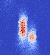
\includegraphics[width=0.28\textwidth]{Zelong_original}};
		\node[lab] at (original.south west) {a};
		\node[pic3d, right=of original] (blurred) {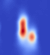
\includegraphics[width=0.28\textwidth]{Zelong_blurred}};
		\draw (blurred.north west) ++(0.0028\textwidth, -0.0028\textwidth)%
			+(0.12481989\textwidth,  -0.12945125\textwidth) circle[radius=0.02524086\textwidth]
			+(0.1244735\textwidth,  -0.17347244\textwidth) circle[radius=0.02491653\textwidth]
			+(0.17678062\textwidth,  -0.20280568\textwidth) circle[radius=0.03129688\textwidth];
		\node[lab] at (blurred.south west) {b};
		\node[pic3d, right=of blurred] (deconvolved) {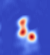
\includegraphics[width=0.28\textwidth]{Zelong_deconvolved}};
		\draw (deconvolved.north west) ++(0.0028\textwidth, -0.0028\textwidth) %
			+(0.12353147\textwidth,  -0.12286225\textwidth) circle[radius=0.02143669\textwidth]
			+(0.12275197\textwidth,  -0.1833389\textwidth) circle[radius=0.02124992\textwidth]
			+(0.17789003\textwidth,  -0.20213276\textwidth) circle[radius=0.02612742\textwidth];
		\node[lab] at (deconvolved.south west) {c};
	\end{tikzpicture}
	\caption{\textbf{Deconvolution.} Detail of the same $YZ$ slice of \textbf{a} original confocal image ($y$), \textbf{b} previous blurred by $\sigma_0=1.6$ ($y_0$) \textbf{c} previous deconvolved by measured kernel (see text). Circles indicate the tracked particles position and size when using whether \textbf{b} or \textbf{c} as first Gaussian layer $G_0$.}
	\label{fig:deconv}
\end{figure}

\end{document}